\documentclass{ieeeaccess}
\usepackage{cite}
\usepackage{amsmath,amssymb,amsfonts}
\usepackage{algorithmic}
\usepackage{graphicx}
\usepackage{textcomp}
\usepackage{changes}
\usepackage{xcolor}
\usepackage{color, soul}
\definecolor{yellow}{rgb}{1.,1.0,0}

\def\BibTeX{{\rm B\kern-.05em{\sc i\kern-.025em b}\kern-.08em
    T\kern-.1667em\lower.7ex\hbox{E}\kern-.125emX}}
\begin{document}
\history{Date of publication xxxx 00, 0000, date of current version xxxx 00, 0000.}
\doi{10.1109/ACCESS.2017.DOI}

\title{Autoencoder-combined Generative Adversarial Networks for Synthetic Image Data Generation and Detection of Jellyfish Swarm}
\author{\uppercase{Kyukwang Kim}\authorrefmark{1}, \IEEEmembership{Student Member, IEEE},
\uppercase{, and Hyun Myung}.\authorrefmark{1},
\IEEEmembership{Senior Member, IEEE}}
\address[1]{Urban Robotics Laboratory, Korea Advanced Institute of Science and Technology, Daejeon 34141, South Korea.}

\tfootnote{This work was partially supported by Korea Minister of Ministry of Land, Infrastructure and Transport (MOLIT) 
through a U-City Master and Doctor Course Grant Program. This work was also supported by the ICT R\&D program of MSIP/IITP. 
(2016-0-00563, Research on Adaptive Machine Learning Technology Development for 
Intelligent Autonomous Digital Companion) and 
National Research Foundation of Korea (NRF) grant funded by the Korea government (MSIP) (NRF-2015R1A2A1A15056262).''}

\markboth
{Author \headeretal: Preparation of Papers for IEEE TRANSACTIONS and JOURNALS}
{Author \headeretal: Preparation of Papers for IEEE TRANSACTIONS and JOURNALS}

\corresp{Corresponding author: Hyun Myung (hmyung@kaist.ac.kr).}

\begin{abstract}
Image-based sensing of jellyfish is important as they can cause great damage to the fisheries and seaside facilities and need to be properly controlled. In this research, we present a deep-learning-based technique to generate a synthetic image of the jellyfish easily with autoencoder-combined generative adversarial networks. The proposed system can easily generate simple images with smaller number of datasets compared to other generative networks. The generated output showed high similarity with the real image dataset. The application using a fully convolutional network and regression network to estimate the size of the jellyfish swarm was also demonstrated, and showed high accuracy during the estimation test.
\end{abstract}

\begin{keywords}
Autoencoder, Generative Adversarial Networks, Jellyfish swarm, Fully Convolutional Network, Regression
\end{keywords}

\titlepgskip=-15pt

\maketitle

\section{Introduction}
\label{sec:introduction}
\PARstart{J}{ellyfish} rapidly proliferate and form a giant swarm in a nutrient-rich environment [1]. Recent changes in the ocean environment, such as global warming and pollution, generated conditions conducive to the jellyfish swarm by decreasing the potential predators of the jellyfish [2]. The huge population of jellyfish has caused great damage to various industries. Fisheries suffer greatly as the jellyfish swarm damages fishing grounds, aqua farms, and fishing tools such as nets [3]. Seaside power plants and resorts also spend a significant amount of their budget to remove jellyfish swarms. In the Republic of Korea, more than 500 cases of human injury and financial damages estimated to be about 135--280 million US dollars occur annually [4].
Many engineering solutions were developed to detect and remove jellyfish swarms. A screening method to clear jellyfish from the cooling water intake channel of the seaside power plants was developed [3]. Some researchers developed a jellyfish-removing robotic system to detect jellyfish population with a quadcopter platform and removing them with co-operating robotic boats [5, 6].

Image recognition plays a key role in the robotic jellyfish-control system. Detecting the moving jellyfish swarm and coordinating the robots to the place where the jellyfish are found allows the efficient and appropriate operation of the robotic system [5]. In addition, the detection system could be used as an alerting system for seaside resorts. Deep architectures used in these image-recognition systems have shown great advances in recent years, accomplishing several improvements in various tasks [7]. However, deep learning requires a large amount of quality-controlled data and manually labeled ground-truth answers to be trained. The jellyfish tend to be sensitive to the temperature and salinity of the water; it is difficult to predict the appearance of the jellyfish and collect the image data for the deep-learning system. Labeling and classification of the collected image data is also a labor-intensive and challenging job. To solve this issue, a generative model will be exploited to generate the image data for training image sensors in this paper.

\Figure[t](topskip=0pt, botskip=0pt, midskip=0pt)[width=\linewidth]{evgan_fig1.png}
{Overall architecture of the proposed image-generation model. The blue solid line shows the dataflow at the train phase. The red dotted line only works at the test phase.\label{fig1}}

Generative Adversarial Networks (GAN), an implicit generative model proposed by Goodfellow \textit{et al}. [8], has attracted the most attention recently. The key feature of the GAN architecture is the two sub-architectures it is composed of the generative network that generates the image from the seed vector and the discriminator network that classifies the generator-synthesized fake images from the real images. These two networks finally optimize the output images as they compete with each other during the training phase; the generator tries to maximize its acceptance ratio (create a realistic image), while the discriminator attempts to minimize the generator output (find every fake image). However, this min-max saddle-point optimization process easily fails and makes it difficult to accomplish the training process of the GAN. Many GAN architectures such as Unrolled-GAN [9] have been proposed to increase the GAN\textquotesingle s stability; however, it is difficult to directly apply these complex structures to previously established systems, or they require a large volume of training data to update the deep structures properly. Research conducted with benchmark datasets such as the MNIST does not suffer from a lack of the data; however, it works as a big entry barrier for applications based on custom datasets. Though the purpose of the GAN is to increase the number of data, a contradictory situation, that GAN requires large number of data occurs.

In this article, we propose a modified GAN structure to reduce the level of image synthesis difficulty. The overall structure of the proposed AE-combined GAN is shown in Fig. 1. We focused on the fact that the autoencoders (AEs) could project a large matrix (image) into a smaller dimension by encoding it. The pre-trained autoencoder-encoded vectors of the real images are trained to the GAN at the train phase and GAN-generated vectors (generated vectors in Fig. 1) are converted to the final image output by the decoder part of the autoencoder. Then the GAN can synthesize new images by generating only short vectors (test phase of Fig. 1), which is much easier than composing entirely new images. The next section also describes how the proposed system can be used to train the image sensor for jellyfish detection in the marine environment.



\section{AUTOENCODER-COMBINED GAN}

\subsection{GAN structure and implementation}

For the implementation, the original multilayer perceptron (mlp) GAN structure used by Goodfellow \textit{et al}. was used. The TensorFlow-based GAN source code available in the Github project was used as a basis code [10]. Both the generator and discriminator of the GAN consist of three layers. The network structural settings of the used AE and GAN are illustrated in Fig. 2. 

\Figure[t](topskip=0pt, botskip=0pt, midskip=0pt)[width=\linewidth]{evgan_fig2.png}
{(a) Layer information of the used autoencoder (AE). The layers named with \textquotesingle neuron\textquotesingle\, indicate the sigmoid layers and the others mean innerproduct (ip) layers. The number written next to the ip layer indicates the product size of the ip layer (e.g. enc2 is 1000x500). (b) Structure and dimension information of the used GANs. Big red arrow pointing enc3neuron indicates the layer where encoded vectors are extracted.\label{fig2}}

The learning rate (lr) of 0.001 without the decay (by setting the step size option larger than the maximum iteration) was used for the optimizer. The weight decay of 0.0005 and the momentum value of 0.9 were used (default values for the MNIST training). With these options, about 5,000 iterations were conducted to optimize the network. The loss per every 100 steps was monitored to check proper termination time. Other detailed options are available online at the Caffe Github [11, 12]. 

The encoded vectors (the enc3neuron in Fig. 2(a)) were used for the GAN training data as mentioned above. The vectors extracted from the sigmoid layer (\textquotesingle neuron\textquotesingle\, layer) showed the better results in the GAN training, and the enc3neuron values were used as it is the deepest neuron layer before the decoding starts. Before training, all training datasets were normalized to fit all values between -1 and 1. The Euclidean loss function combined with the RMSprop optimizer used in the LSGAN was applied [13]. The GANs generally use sigmoid-cross entropy losses to check a probability that with the given input, the discriminator is real or not. However as the generated outputs of the proposed GAN are size-reduced vectors instead of the image, we used the Euclidean loss, which measures the spatial distance from the training datasets for higher differentiability between the generated vectors and real vectors.

\subsection{Training image preparation}
The video of the jellyfish swarm proliferating in the sea near the cities of Changwon and Masan, Republic of Korea was recorded. The raw images of the ocean scene with the size of $1080 \times 980$ were collected by the Logitech c920r camera attached to the Unmanned Aerial Vehicle (UAV) hovering about 4 to 5m from the water surface. At this altitude, the adult Aurelia aurita, the jellyfish species which is the main cause of the jellyfish bloom, fits within the $32 \times 32$ square image patches. One hundred jellyfish image patches [16] were manually cropped and classified from the captured video. The background seawater image of each patch was removed and changed into a plain black background. All jellyfish images were converted into grayscale before training to reduce the diversity within the dataset as much as possible. The real exemplary ocean scene and the jellyfish patch are shown in Fig. 3.

\Figure[t](topskip=0pt, botskip=0pt, midskip=0pt)[width=0.8\textwidth]{evgan_fig3.png}
{The jellyfish blooming real ocean scene image taken by the UAV and background removed image patch used for the training.\label{fig3}}

\Figure[!t](topskip=0pt, botskip=0pt, midskip=0pt)[width=\linewidth]{evgan_fig4.png}
{Flow diagram of the jellyfish swarm size level regression system. (a) Generating synthetic jellyfish images from the real jellyfish patches, generating an 
artificial scene. (b) FCN training with the synthetic scene. (c) Regression of the probability score map obtained by processing the real seawater scene into the synthetic-image-trained FCN.\label{fig4}}

\subsection{Synthetic-image-based fully convolutional network training.}
The fully convolutional network (FCN) is a network used for the semantic segmentation of the image [17]. This network calculates the pixel-wise association probability and generates a contour-like probability map of the labeled data on the image. This network can infer much higher pixel-wise resolution classification results compared to the bounding box inference or simple whole-image classification network. The FCN is also combined with the regression neural network to obtain regression results such as object counting by using the FCN-generated probability map as an input [18]. Despite this usefulness, preparing the label data for the FCN  is the most labor-intensive compared to other classification networks. The target objects in the original image should be carefully colored to obtain the boundary region clearly. Other non-target objects should be removed and changed into the background color. At least a few hundred images should be processed to train the simplest FCN. If the target object is a vague jellyfish-like object in the water, the labeling process becomes more difficult.

In this paper, we use the GAN-generated synthetic image to solve the addressed issue. The synthetic jellyfish images generated by the GAN were attached to random points of the seawater image. As the exact point, size, and contour boundary of the synthetic patches are known, the black-and-white label image can be prepared automatically during the synthetic-scene generating process.

In the Republic of Korea, the jellyfish alert given by the National Institute of Fisheries Science (NIFS) is classified into three levels (excluding \textquotesingle attention\textquotesingle\, level which indicates that a new jellyfish polyp colony was found) [19]. The regression class was classified into three labels to mimic this alert system; the \textquotesingle clear\textquotesingle\, level indicating the low density of the jellyfish (about 0 to 5 jellyfish), the \textquotesingle advisory\textquotesingle\, level which means the medium swarm size (more than 20), and the \textquotesingle alert\textquotesingle\, level notifying severe bloom of the swarm (about or more than 100). The exact alert is given by counting the actual numbers within a $10 m \times 10 m$ area. However, as the recorded video did not contain flight odometry data, we only mimicked a three-level differentiation of the jellyfish swarm\textquotesingle s density and approximate jellyfish numbers. In our experiment, random numbers (1 - 10, 20 - 40, and 70 - 100) of the random jellyfish patches were placed on the blank seawater scene (no jellyfish in the ocean) and 100 synthetic scenes and labels were generated.

The FCN was trained by the synthetic scene for about 1,300 iterations (learning rate of 0.0001 with the decay function drops to near zero at this point). After the pre-trained FCN was prepared, 100 real seawater scenes (real jellyfish exists) were passed to the pre-trained FCN to obtain the probability score map. The collected score map was classified into three density levels based on the original jellyfish number in the original real scene and trained to the regression network. An AlexNet structure with the Euclidean loss and single regression output final node were applied to the regression process (learning rate of 0.001, 6000 iteration). The overall process is shown in Fig. 4.

\section{RESULTS AND DISCUSSION}

\subsection{Synthetic jellyfish image generation}
The synthetic jellyfish images were generated by the proposed GAN architecture. For a comparison, the basic mlp GAN, Deep Convolutional GAN (DCGAN) [20], and Boundary Equilibrium GAN (BEGAN) [21] were chosen. The DCGAN showed good results in various benchmark datasets and its implementation code [22] has been applied to many open-source GAN implementation projects. BEGAN is one of the most cutting-edge, recently published GAN structures famous for its high-resolution generative ability. The open-source implementation of BEGAN [23, 24] was used for the test. \hl{Structure information of the used GANs is shown in Table 1. The exhaustive grid search method [25] was used to find best training options of the tested GANs. A set of hyper-parameter values such as the learning rate , optimizer, and batch size were selected and the each combination of these parameters was tested. The values used are determined empirically, or by reference to existing values or values given by the available codes. All combinations were trained for 100 epochs and generated output of every epoch was monitored to find the optimized point. The parameters at the optimized states are shown in Table 2.} The generated image outputs are shown in Fig. 5. 

\Figure[!t](topskip=0pt, botskip=0pt, midskip=0pt)[width=0.7\linewidth]{fig_5_2.png}
{Generated image outputs and comparison with the real image. (a) Basic mlp GAN (b) DCGAN (c) BEGAN (d) Proposed AE-combined mlp GAN and (e) Real jellyfish image.\label{fig5}}

\begin{table}
\caption{Used GANs structure information}
\label{table}
\setlength{\tabcolsep}{3pt}
\begin{tabular}{|p{40pt}|p{200pt}|}
\hline
Network $^{\mathrm{a}}$ & 
Structure $^{\mathrm{b}}$ \\
\hline
MLP G& 
$100\times 150 fc-150\times 300 fc - 300\times 1024 fc$  \\
MLP D& 
$1024\times 300 fc-300\times 150 fc - 150\times 1 fc$ \\
DC G& 
$100\times 512 dc-512\times 256 dc - 256\times 128 fc- 128\times 64 dc- 64\times 3 dc$  \\
DC D& 
$3\times 64 c-64\times 128 c - 128\times 256 c- 256\times512 c- 512\times 1 c$ \\

BE G& 
$64\times (64 \times 32 \times 32) fc-(CIE-CIE-U) \times 4-CIE- 64\times 3 c$ \\

BE D enc& 
$3\times 64 c- CIE 1\times2- CIE 2\times2- CIE 2\times3- CIE 3\times3- CIE 3\times4- CIE 4\times4- CIE 4\times5- CIE 5\times5$ \\

BE D dec& 
$ CIE-U-(CIE-CIE-U) \times 3 - CIE- 63\times 3 c $ \\

BE D& 
BE D enc $- (64\times5\times32\times32)\times 64 fc - 64\times (64\times32\times32) fc$ - BE D dec\\

\hline
\multicolumn{2}{p{251pt}}{$^{\mathrm{a}}$
G$=$Generator structure of the given GANs. D$=$Discriminator structure of the given GANs. BE D enc$=$ Encoder module of BEGAN discriminator. BE D dec$=$ Decoder module of BEGAN discriminator.  }\\
\multicolumn{2}{p{251pt}}{$^{\mathrm{b}}$
$(n \times m)fc = $ $n$ by $m$ fully connected layer. $(n \times m)dc = $ $n$ by $m$ deconvolution layer. $(n \times m)c = $ $n$ by $m$ convolution layer. $CIE  = 64\times64$ convolution layer, 2D instance norm-exponential linear unit, and  exponential linear unit(ELU) activation layer compound. $CIE (i \times j)=$ $i \times 64$ by $j \times 64$ convolution layer CIE unit. $U=$ upsample layer.}
\end{tabular}
\label{tab1}
\end{table}

\begin{table}
\caption{Training hyper-parameters of the GANs.}
\label{table}
\setlength{\tabcolsep}{3pt}
\begin{tabular}{|p{45pt}|p{40pt}|p{40pt}|p{40pt}|p{40pt}|}
\hline
& 
GAN& 
DCGAN&
BEGAN&
Proposed\\

\hline
Learning rate & 
$0.0001 $& 
$0.0002 $& 
$0.0008 $& 
$0.001 $\\
Batch size& 
$16 $& 
$16 $& 
$16 $& 
$16 $\\
Optimizer& 
Adam& 
Adam& 
Adam& 
RMSprop\\
Train epoch& 
$100 $& 
$90 $& 
$50 $& 
$70 $\\
Train result$^{\mathrm{a}}$& 
$\times$& 
$\circ$& 
$\times$& 
$\circ$\\

\hline
\multicolumn{5}{p{233pt}}{$^{\mathrm{a}}$
Indicates whether the GAN successfully trained or showed mode collapse.}\\
\end{tabular}
\label{tab1}
\end{table}

\hl{The results showed that the classic GAN could not generate any image; only dot-like figures were observed though many trials were done. A phenomenon called mode collapse, where only identical images are generated at one test batch, was observed during the test using the classic GAN. The DCGAN showed much better performance. The DCGAN generated jellyfish-like figures. Some image patches showed quite good results; however, the overall texture and brightness were very rough compared to the real images. Also, wrong combination of the learned features was observed. Though some part of the generated image resembles the real image, the whole image becomes awkward as the assembled image does not look like a jellyfish. The BEGAN showed the best realities in the texture generation but failed to generate the images and showed mode collapse. Under limited dataset size conditions, suitably training the deep structures of the BEGAN was hard and shallow GANs such as the DCGAN showed the better results.} Compared to the previous methods, the proposed AE-combined GAN generated more successful results. The synthetic image still lacked details compared to the original dataset. The inner texture of the jellyfishes was not fully reconstructed. However, the proposed method successfully generated round and smooth elliptical shapes, which is a much better result compared to the conventional methods. For a quantitative comparison, the cosine similarity and mean squared errors (MSE) of the test-batch output of each GAN were compared with the real dataset. Ten batch outputs were selected and compared with the whole train data. The maximum cosine similarity and the minimum MSE (best cases) value per comparison were collected. \hl{For the establishment of the standard value, 5 random images were selected from the real image and the same error computation was performed. The results are summarized in Table 3.}



\begin{table}
\caption{Mean squared errors and cosine similarity of the generated image compared with the real data.}
\label{table}
\setlength{\tabcolsep}{3pt}
\begin{tabular}{|p{30pt}|p{75pt}|p{115pt}|}
\hline
Method& 
Minimum MSE& 
Maximum cosine similarity \\
\hline
GAN & 
$13.31 \pm 1.46$& 
$0.702 \pm 0.043$ \\
DCGAN& 
$40.81 \pm 6.87$& 
$0.90 \pm 0.057$ \\
BEGAN& 
$68.32 \pm 3.5$& 
$0.91 \pm 0.02$ \\
Proposed& 
$35.28 \pm 1.40$& 
$0.94 \pm 0.02$ \\
Real& 
$25.55 \pm 1.40$& 
$0.98 \pm 0.02$ \\

\hline

\end{tabular}
\label{tab1}
\end{table}

\hl{The proposed method showed the second-best MSE result and the best cosine similarity result compared to the other conventional methods excluding the real data. The original mlp GAN showed an abnormally low MSE error (even lower than the real data sampled result) because of the matching between black backgrounds of the original images. The DCGAN showed good results in both the cosine similarity and the MSE as it generated jellyfish like figure though texture was rough. The BEGAN showed good cosine similarity score due to low difference in the generated image pool. As the best cases are collected, if all the images look similar due to the mode-collapse, the similarity value tends to be fixed though the quality of the image is bad. A lower MSE value of the proposed method compared to the real dataset shows a slight lack of inner diversity of the generated output, and needs to be improved.}

The single jellyfish patch is only a $32 \times 32$ sized object. The image of the jellyfish was taken with the gimbal-mounted camera of a quadcopter platform. Thus, the image was very small and blurred compared to the other benchmark datasets. We assume that the DCGAN-based modern GANs failed because it could not find the appropriate features to learn from the given jellyfish datasets. Excessively simple shapes of the train images caused bad results in complex structured neural networks. The merits of the AEs can be found in these situations. The AEs can be easily trained; rather small numbers of data are enough to train AEs compared to the GANs. Though the GAN generates a relatively poor output, the AE can project the generated vectors to an image, which helps in increasing the quality of the output images.

The usage of the AEs in the GAN also brings other merits. The AE plays key roles in image generation in the proposed system. As the AE can reconstruct more realistic images from the encoded vectors, the quality of the overall system increases even though the GAN generates the vectors with similar qualities. The output of the GAN is unpredictable before training. However, the proposed system\textquotesingle s output is ensured if the AE-generated images have acceptable qualities.
If the benchmark dataset with many well-qualified images is used, other cutting-edge GAN structures are expected to show competitive performance with the proposed system. However, collecting and labeling data is a costly job, and obtaining sufficient data is sometimes impossible. The proposed method has a comparative advantage over previous methods, as it requires a small number of datasets to generate the data. Further, the jellyfish image differs based on the recording drone\textquotesingle s flying altitude and regions. The requirement of less data indicates that the proposed system can generate a custom image dataset mimicking the recorded condition of different regions more easily as compared to other systems.


\subsection{Jellyfish swarm density level estimation with a synthetic-image-trained network}

The FCN-based regression method is very useful in estimating the distribution of the target objects in the scene with very low computational cost, as it does not require classification (neural network feed-forward computation) of every candidate figure in the image. In this paper, we tested whether the FCN trained with the synthetic ocean scene can generate a good probability score map even though the realistic images are given. The results are shown in Fig. 6.

\Figure[!t](topskip=0pt, botskip=0pt, midskip=0pt)[width=0.8\linewidth]{evgan_fig6.png}
{Real ocean scene and probability map generated by the synthetic image pre-trained FCN. The pale white dots in the ocean scene images are real jellyfishes. (a) Low level of jellyfish density (clear). (b) Medium level of jellyfish density (advisory). (c) High level of jellyfish density (alert).\label{fig6}}

Hundred real ocean images were classified into three classes based on the number of the jellyfish in the image. The three level criteria was used to mimic actual jellyfish swarm alert criteria explained in Section 2.3.

The accuracy of the regression network was measured after processing test datasets, which was not used during the training phase. The results showed an accuracy of 83.8\%; total 52 correct classifications were obtained among 62 test data. \hl{The previous research on classifying jellyfish image patch with the deep-learning architecture showed 80.5\% accuracy [6].} Though the final target is slightly different, the obtained accuracy gave acceptable results compared to the previous research. In the case of the number regression, the counting method using the classification of every object candidate in the image shows a relatively low accuracy even though the classification accuracy is high (over 80\%). If there are number of objects in the image, even a very accurately trained classifier can output a high error rate due to multiple classification operations in a single image. The FCN combined with the regression networks shows better performance in this case as it can locate possible targets at a single inference. 

\hl{For further comparison, the same real jellyfish bloom scene images used was manually labeled and used as the train dataset for the FCN network. The processes shown in Fig. 4(b) and Fig. 4(c) were repeated by the human labeled train data to compare with synthetic image based results. The real image trained regression network showed the accuracy of 71.4\%. The proposed synthetic jellyfish based method showed better results even though the real jellyfish scene was labeled and given as a train input to the network. Though labeled by human labors, the labeled data is not perfect and even the pixel-wise errors can confuse the FCN during the training phase. This phenomenon is more noticeable when the size of the data increases and the data is distributed to the many workers as the labeling criteria differ among workers. The synthetic data is much more free on this issue as near-perfect label can be generated. The amount of the data also plays important rule in the accuracy of the deep neural networks. Synthetic data based method can easily increase the number of the labeled data with much less cost compared to the real data which requires human labor to be labeled.}

The proposed synthetic-scene-based method can gradually aid overall process by automatically generating labels and features for training the FCNs. Moreover, the dots found in the probability map in Fig. 6 are well-matched with the real jellyfish distribution. These results and the high accuracy with real data show that the synthetic jellyfish image is reasonably similar to the real jellyfish in view of the neural networks.

\section{CONCLUSIONS AND FUTURE WORK}
This paper presented a newly developed technique using the AE and GAN to solve the image generation issue in a small-numbered, simple-featured image dataset. The jellyfish was used as an example to show that the proposed method successfully works in cases that cannot be solved by using conventional GANs. The training of the deep-learning-based jellyfish swarm density level estimation with the synthetic image was shown as an application of the proposed method to realistic problems. 

As future work, we are considering the upgrade of the autoencoder\textquotesingle s image restoration ability by applying more sophisticated autoencoders, such as the deep convolutional autoencoder. The autoencoder-generated vectors, which are used as a training input to the GAN, are rather closer to a sequence than an image. We are considering the application of sequence-specific GANs to increase the GAN\textquotesingle s functionalities. Further application of the proposed GAN structure to other image datasets [26], is also under consideration.


\begin{thebibliography}{00}

\bibitem{b1} M. N. Arai, \textit{A functional biology of Scyphozoa}, London, UK, Chapman \& Hall, 1997, pp. 316.

\bibitem{b2} J. E. Purcell and M. N. Arai, ``Interactions of pelagic cnidarians and ctenophoors with fish: a review,'' \textit{Hydrobiologia}, vol. 451, pp. 27--44, 2001.

\bibitem{b3} Ministry of Land, Infrastructure and Transport (MOLIT), Republic of Korea. ``Hazardous marine life jellyfish damage prevention research projects,'' 2012.

\bibitem{b4} B. T. Kim, K. H. Eom, I. S. Han, and H. J. Park, ``An analysis of the impact of climatic elements on the jellyfish blooms,'' \textit{J. Fisheries. Marine. Edu}., vol. 27, no. 6, pp. 1755--1763, 2015.

\bibitem{b5} H. Kim, D. Kim, H. Kim, J. U. Shin, and H. Myung, ``An extended any-angle path planning algorithm for maintaining formation of multi-agent jellyfish elimination robot system,'' \textit{Int. J. Contr. Autom. Syst}., vol. 14, no. 2, pp. 598--607, 2016.

\bibitem{b6} H. Kim, J. Koo, D. Kim, S. Jung, J. U. Shin, S. Lee, and H. Myung, ``Image-based monitoring of jellyfish using deep learning architecture,'' \textit{IEEE Sensors J}., vol. 16, no. 8, pp. 2215--2216, 2016

\bibitem{b7} K. Simonyan and A. Zisserman, ``Very deep convolutional networks for large-scale image recognition,'' arXiv:1409.1556 [cs.CV], Apr. 2015.

\bibitem{b8} I. Goodfellow, J. Pouget-Abadie, M. Mirza, B. Xu, D. Warde-Farley, S. Ozair, A. Courville, and Y. Bengio, ``Generative adversarial networks,'' arXiv:1406.2661 [cs.ML], Jun. 2014.

\bibitem{b9} L. Metz, B. Poole, D. Pfau, and J. Sohl-Dickstein, ``Unrolled generative adversarial networks,'' arXiv:1611.02163 [cs.LG], Nov. 2016.

\bibitem{b10} GAN implementation github page. Accessed on: Nov. 2, 2017. [Online]. Available: \underline{https://github.com/ckmarkoh/GAN-tensorflow/}

\bibitem{b11} Y. Jia, E. Shelhamer, J. Donahue, S. Karayev, J. Long, R. Girshick, S. Guadarrama, and T. Darrell, ``Caffe: Convolutional architecture for fast feature embedding,''  arXiv:1408.5093 [cs.CV], Jun. 2014.

\bibitem{b12} Caffe github page MNIST autoencoder example source code. Accessed on: Nov. 2, 2017. [Online].  Available: \underline{https://github.com/BVLC/caffe/tree/master/examples/mnist/}

\bibitem{b13} X. Mao, Q. Li, H. Xie, R. Lau, Z. Wang, and S. P. Smolley, ``Least squares generative adversarial networks,'' arXiv:1611.04076 [cs.CV], Nov. 2016. 

\bibitem{b14} A. B. L. Larsen, S. S{\o}nderby, H. Larochelle, and O. Winther, ``Autoencoding beyond pixels using a learned similarity metric,'' arXiv:1512.09300 [cs.LG], Dec. 2015. 

\bibitem{b15} A. Makhzani, J. Shlens, N. Jaitly, I. Goodfellow, and B. Frey, ``Adversarial autoencoders,'' arXiv:1511.05644 [cs.LG], Nov. 2015.

\bibitem{b16} Used jellyfish image dataset. Accessed on: Nov. 2, 2017. [Online].  Available: \underline{http://urobot.synology.me/data/evgan\_jellyfish\_img.zip/}

\bibitem{b17} E. Shelhamer, J. Long, and T. Darrell, ``Fully convolutional networks for semantic segmentation,'' arXiv:1605.06211 [cs.CV], May 2017.

\bibitem{b18} S. W. Chen, S. S. Shivakumar, S. Dcunha, J. Das, E. Okon, C. Qu, C. J. Taylor, and V. Kumar, ``Counting apples and oranges with deep learning: A data driven approach,'' in \textit{Proc. IEEE International Conference on Robotics and Automation (ICRA)}, Singapore, 2017, pp. 781--788.

\bibitem{b19} Ministry of Oceans and Fisheries, Republic of Korea. ``Fishery damage due to massive jellyfish occurrence,'' 2014.

\bibitem{b20} A. Radford, L. Metz, and S. Chintala, ``Unsupervised representation learning with deep convolutional generative adversarial networks,'' arXiv:1511.06434 [cs.LG], Nov. 2015.

\bibitem{b21} D. Berthelot, T. Schumm, and L. Metz, ``BEGAN: Boundary equilibrium generative adversarial networks,'' arXiv:1703.10717 [cs.LG], Mar. 2017.

\bibitem{b22} DCGAN implementation github page. Accessed on: Nov. 2, 2017. [Online]. Available: \underline{https://github.com/carpedm20/DCGAN-tensorflow/}

\bibitem{b23} BEGAN implementation github page. Accessed on: Nov. 2, 2017. [Online]. \underline{Available: https://github.com/TuXiaokang/BEGAN.PyTorch/}

\bibitem{b24} BEGAN implementation github page. Accessed on: Nov. 2, 2017. [Online]. \underline{Available: https://github.com/carpedm20/BEGAN-tensorflow/}

\bibitem{b25} J. Zhao, M. Mathieu, and Y. LeCun, ``Energy-based Generative Adversarial Network,'' 	arXiv:1609.03126 [cs.LG], Sep. 2016.

\bibitem{b26} K. Kim, H. K. Kim, H. Lim, and H. Myung, ``A low cost/low power open source sensor system for automated tuberculosis drug susceptibility testing,'' \textit{Sensors}, vol. 16. pp. 942, 2016.

\end{thebibliography}

\begin{IEEEbiography}[{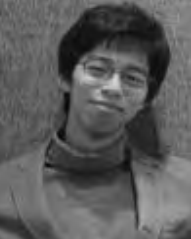
\includegraphics[width=1in,height=1.25in,clip,keepaspectratio]{a1.png}}]{KYUKWANG KIM}
received the B.S. degree in bio and brain engineering from the Korea Advanced Institute of Science and Technology, where he is currently pursuing the M.S. degree with the robotics program. His research includes bioinformatics, biosensors, environmental robotics, and machine learning.
\end{IEEEbiography}

\begin{IEEEbiography}[{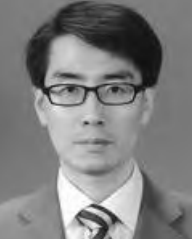
\includegraphics[width=1in,height=1.25in,clip,keepaspectratio]{a2.png}}]{HYUN MYUNG} 
received the B.S., M.S., and Ph.D. degrees from the Korea Advanced Institute of Science and Technology (KAIST), Daejeon, South Korea, in 1992, 1994, and 1998, respectively, all in electrical engineering. He was a Senior Researcher with the Electronics and Telecommunications Research Institute, Daejeon, from 1998 to 2002, a CTO and the Director with the Digital Contents Research Laboratory, Emersys Corporation, Daejeon, from 2002 to 2003, and a Principle Researcher with the Samsung Advanced Institute of Technology, Yongin, South Korea, from 2003 to 2008. Since 2008, he has been an Associate Professor with the Department of Civil and Environmental Engineering, KAIST, where he is currently an Adjunct Professor in robotics program. His current research interests include structural health monitoring using robotics, soft computing, simultaneous localization and mapping, robot navigation, machine learning, deep learning, and swarm robot.  
\end{IEEEbiography}

\EOD

\end{document}
